%------------------------------------------------
%
% Incident.tex 
%
% This section introduces the incident process.
%------------------------------------------------
\section[Incident Management]{incident management}
\label{prc-incident}
Dalla documentazione ufficiale \ac{Information-Technology-Infrastructure-Library} si evince che l'obiettivo primario di questo processo consiste nel ripristinare l'operatività del servizio, al livello concordato con il cliente/utente, a seguito di un incidente assicurando la minima interruzione possibile oppure entro i termini previsti dal documento di \ac{Service-Level-Agreement}.

Spesso, a seguito di un incidente, il ripristino del servizio avviene attraverso l'attivazione di un \english{work around} che permette all'utente di tornare ad essere operativo, possibilmente con un livello di servizio inferiore, fin tanto che il processo di \ac{Problem-Management} non riesce a determinare le cause che hanno scatenato l'incidente al fine di produrre una soluzione.

E' importante osservare che non ha solo lo scopo di ripristinare il servizio ma deve anche tracciare tutte le informazioni che sono a corredo dell'incidente.


\subsection[Differenza tra incidenti e problemi]{differenza tra incidenti e problemi}
\label{prc-incident-versus-problem}
In ambiente \ac{Information-Technology-Infrastructure-Library} un incidente ed un problema assumono significati differenti anche se gli utenti spesso li confondono o li percepiscono come la stessa entità.

Un \keyword{incidente} accade quando qualcosa, generalmente un \ac{Configuration-Item}, non lavora come dovrebbe; spesso è descritto dagli utenti come:

\begin{itemize}
\item{un guasto;}
\item{un errore.}
\end{itemize}

Generalmente esso impedisce l'accesso al servizio, o lo garantisce in modo ridotto, ad un singolo utente.

Un \keyword{problema} invece è differente, e può essere:

\begin{itemize}
\item{l'occorrenza dello stesso incidente molteplici volte;}
\item{un incidente che influisce su molti utenti;}
\item{il risultato di una diagnosi di rete che rivela la non operatività normale di qualche sistema.}
\end{itemize}

La gestione dei problemi differisce dalla gestione degli incidenti in quanto possiede un obiettivo diverso; essa mira a capire le cause scatenanti dell'incidente invece che pensare ad un rapido ripristino del servizio. Può capitare quindi che gli obiettivi del processo di \ac{Incident-Management} e di \ac{Problem-Management} siano in netto contrasto tra di loro.

Un possibile approccio, per far coesistere entrambi, può essere quello di ripristinare il servizio il più presto possibile (\ac{Incident-Management}), assicurando che tutti i dettagli siano tracciati correttamente. Questo consente di attivare il processo di \ac{Problem-Management} a proseguire nella ricerca della causa, finché è attivo un \english{work around}.

In conclusione, un problema può esistere senza avere un impatto immediato sugli utenti, mentre invece un incidente è di solito maggiormente visibile e ha un impatto maggiore sugli utenti del servizio.

\subsection[Tipologie di incidenti]{tipologie di incidenti}
\label{prc-incident-typology}
Gli incidenti \acs{Information-Technology} che accadono all'interno di una struttura non sono tutti del medesimo tipo, ma posso essere raggruppati in due macro tipologie.

Esse sono:

\begin{itemize}
\item{incidenti utente, suddivisi in:}
\begin{itemize}
\item{incidenti di applicazione}
\item{incidenti \english{hardware}}
\end{itemize}
\item{incidenti tecnici}
\end{itemize}

Viene ora fornita una breve panoramica su entrambe le tipologie.

\subsubsection[Incidenti utente]{incidenti utente}
In questa tipologia si trovano gli incidenti che sono maggiormente incontrati dagli utenti durante l'uso dei servizi \acs{Information-Technology}.

Negli incidenti di applicazione ritroviamo per esempio:

\begin{itemize}
\item{servizio non disponibile;}
\item{visualizzazione di un messaggio di errore quando l'utente prova ad accedere all'applicazione;}
\item{errore di programmazione che impedisce all'utente di proseguire nelle proprie mansioni;}
\item{spazio su disco esaurito.}
\end{itemize}

Invece negli incidenti \english{hardware} ritroviamo per esempio:

\begin{itemize}
\item{il \acs{Personal-Computer} non si accende;}
\item{la stampante non esegue le stampe;}
\item{nuovo \english{hardware} installato che non funziona correttamente.}
\end{itemize}

\subsubsection[Incidenti tecnici]{incidenti tecnici}
Gli incidenti tecnici posso accadere senza che l'utente ne sia consapevole. Potrebbe esserci, per esempio, una risposta più lenta della rete o su una specifica \english{workstation} ma, finché il declino è graduale, l'utente potrebbe non notarlo.

Lo staff tecnico del \english{Service Desk} usando strumenti di diagnostica o di monitoraggio pro attivo è in grado di individuare incidenti tecnici. Se un incidente tecnico non è risolto al più presto può impattare molti utenti per molto tempo.

Con il tempo, e con l'esperienza, il personale del \english{Service Desk} può individuare e risolvere questa tipologia di incidenti prima che impattino su molti utenti.

Esempi di incidenti tecnici possono essere:

\begin{itemize}
\item{spazio su disco quasi esaurito;}
\item{scheda di rete con funzionamento ad intermittenza;}
\item{sfarfallio del monitor (più accentuato in alcune applicazioni).}
\end{itemize}

\subsection[Perché avere un processo di IM]{perché avere un processo di IM}
\label{prc-why-im-process}
Avere nel proprio istituto un processo di \ac{Incident-Management} offre i seguenti benefici:

\begin{itemize}
\item{migliore informazione ai clienti/utenti sugli aspetti della qualità del servizio;}
\item{migliore informazione sull'affidabilità delle apparecchiature;}
\item{miglior sicurezza personale sul fatto che esiste un processo che si occupa dell'operatività dei servizi;}
\item{la certezza che gli incidenti saranno affrontati e non dimenticati;}
\item{riduzione dell'impatto degli incidenti sul \english{business} dell'organizzazione;}
\item{anteporre la risoluzione dell'incidente a quella del problema;}
\item{operare essendo consapevoli della configurazione e di eventuali modifiche al sistema;}
\item{miglior controllo e capacità di interpretare le relazioni, il che contribuisce ad individuare possibili incidenti prima che impattino sugli utenti.}
\end{itemize}

I seguenti benefici si ottengono solamente con un processo di \ac{Incident-Management} correttamente configurato, con i compiti e le attività di lavoro chiaramente definite. Altrimenti si corre il rischio che:

\begin{itemize}
\item{nessuno gestisca o scali gli incidenti;}
\item{vi sia una superflua severità degli incidenti ed una maggiore probabilità di impatto su altri settori;}
\item{ai tecnici viene richiesto di eseguire (spesso) lavori di \english{routine} (es. caricare il vassoio della carta della stampante);}
\item{il personale dello staff potrà essere oggetto di costanti interruzioni che lo rendono meno efficace;}
\item{frequente analisi di incidenti simili piuttosto che fare rifermento a soluzioni esistenti nella \ac{Knowledge-Base};}
\item{mancanza di informazioni di coordinazione tra i membri dello staff;}
\item{incidenti dimenticati o mal gestiti.}
\end{itemize}

\subsection[Input del processo di IM]{input del processo di IM}
\label{prc-incident-inputs}
Il processo di \ac{Incident-Management} riceve \english{input} da diverse sezioni del \english{framework} \ac{Information-Technology-Infrastructure-Library} oltre che dagli utenti dei servizi.

E' una situazione comune che i processi richiedano informazioni in \english{input} da diversi altri processi in quanto il \english{framework} non predilige gli aggregati di informazione ma più piuttosto predilige l'informazione condivisa affinché tutti ne possano trarre beneficio.

Riceve input:

\begin{itemize}
\item{dagli utenti/clienti;}
\item{dal processo di \ac{Problem-Management};}
\item{dal processo di \ac{Change-Management};}
\end{itemize}

\subsubsection[Input dagli utenti]{input dagli utenti}
L'utente/cliente quando scopre di avere un disservizio in corso effettua una richiesta di assistenza presso il \english{Service-Desk} attraverso l'apertura di un \glossarySingolarTerm{ticket} sull'apposito canale di comunicazione (vedi Sezione \ref{sd-contact-mode}).

La richiesta di assistenza, il \english{ticket}, è composto da diverse sezioni con relativi dati tecnici (vedi Sezione \ref{prc-incident-ticket}) che hanno lo scopo di fornire tutte le informazioni necessarie alla prima linea di supporto affinché possa ripristinare il servizio oppure avviare le dovute analisi alla ricerca della/le causa/e scatenanti.

\subsubsection[Input dal processo di PM]{input dal processo di PM}
Affinché un servizio possa essere ripristinato velocemente è utile per lo staff tecnico del \english{Service Desk} avere informazioni su incidenti o su errori precedenti.

Queste informazioni sono reperibili all'interno del \ac{Known-Error-DataBase} e vi sono riposte dallo stesso staff del \english{Service Desk} dopo che il processo di \ac{Problem-Management} ha eseguito le sue mansioni ed ha fornito i dettagli in merito alle cause scatenanti e la risoluzione del problema.

\subsubsection[Input dal processo di CM]{input dal processo di CM}
Quando un \ac{Configuration-Item}/servizio non è configurato nel modo opportuno, il processo di \ac{Incident-Management} esegue una richiesta al processo di \ac{Change-Management} affinché si possa modificare.

Al termine delle attività del processo di \ac{Change-Management} esso fornisce una risposta in merito alla fattibilità o meno della modifica richiesta. Questo consentirà allo staff di aggiornare il \ac{Configuration-Management-DataBase} e, possibilmente, informare l'utente che può aver indirettamente richiesto la modifica.

In caso di futuri incidenti lo staff tecnico consultando il \ac{Configuration-Management-DataBase} può sempre conoscere l'attuale configurazione dell'ambiente e capire se vi sono state modifiche di recente, poiché modifiche all'ambiente \acs{Information-Technology} possono essere la causa di incidenti.

\subsection[Output del processo di IM]{output del processo di IM}
\label{prc-incident-output}
Il processo di \ac{Incident-Management} al termine delle sue attività fornisce, sempre, degli \english{output} che possono essere utilizzati come base di partenza per attivare altri processi.

I suoi \english{output} non sono solo rivolti ad altri processi presenti nel \english{framework} ma sono principalmente rivolti agli utenti/clienti che hanno aperto richieste di assistenza/aiuto. Poiché è suo compito mantenere gli utenti/clienti costantemente aggiornati quando qualcosa di significativo accade sulle loro richieste.

I suoi output sono i seguenti:

\begin{itemize}
\item{dettagli di risoluzione dell'incidente;}
\item{aggiornamento del registro delle chiamate e degli incidenti;}
\item{\english{work around};}
\item{comunicazione con gli utenti del servizio;}
\item{richieste di modifica al servizio (\ac{Request-For-Change});}
\item{stesura di report sul processo;}
\item{input per il processo di \ac{Problem-Management}.}
\end{itemize}

\subsection[Attività del processo di IM]{attività del processo di IM}
\label{prc-incident-activities}
Il processo di \ac{Incident-Management} esegue varie attività dopo che una richiesta di assistenza è giunta ad esso e tutte concorrono alla risoluzione finale dell'incidente.

Tra le attività troviamo:

\begin{itemize}
\item{rilevamento e registrazione dell'incidente;}
\item{fornitura del supporto iniziale;}
\item{investigazione e diagnosi;}
\item{risoluzione e recupero;}
\item{chiusura dell'incidente;}
\item{\english{ownership} dell'incidente, monitoraggio e comunicazione.}
\end{itemize}

In Figura \ref{prc-incident-activities-img} è presente un diagramma di flusso che lega insieme le varie attività presenti nel processo mentre le successive sezioni illustrano nel dettaglio le varie attività. Si parte da una richiesta in ingresso, che può giungere da diversi canali, fino ad arrivare alla sua conclusione.

\begin{figure}[htbp]
\centering
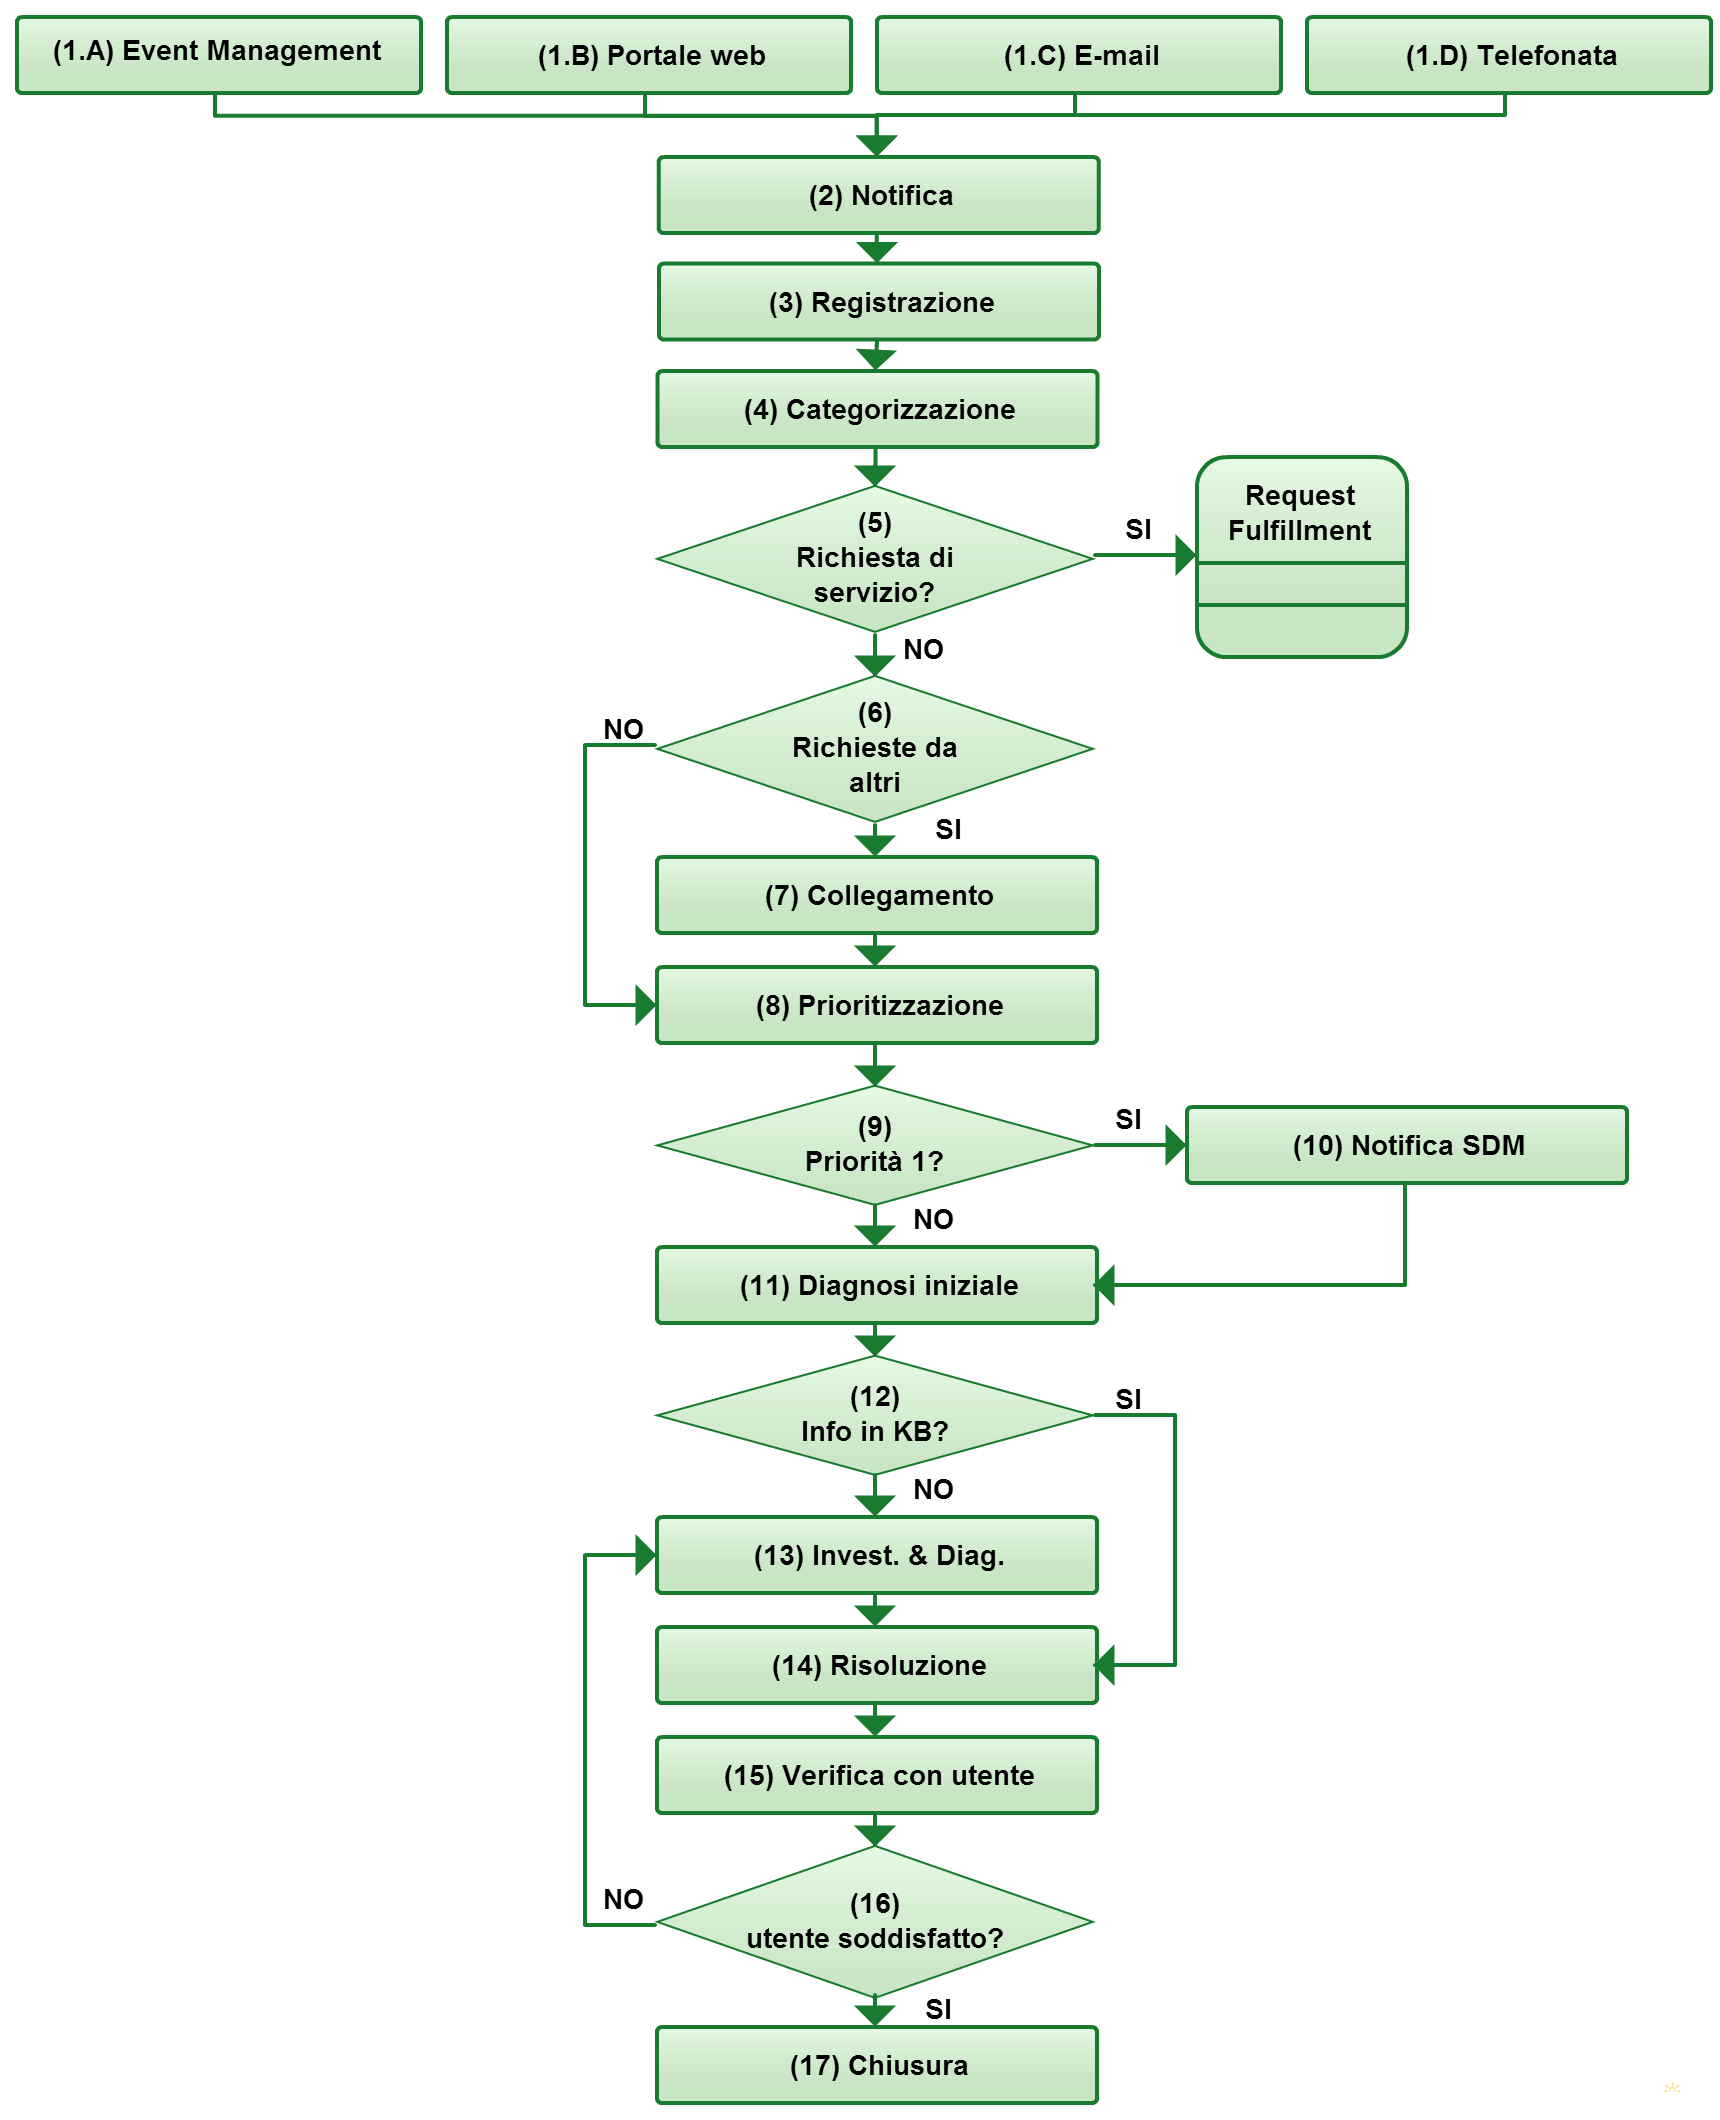
\includegraphics[scale=0.25]{Images/Diagrams/IncidentManagement.png}
\caption{Flusso di lavoro del processo di \ac{Incident-Management}}
\label{prc-incident-activities-img}
\end{figure}

\subsubsection[Rilevamento Registrazione Categorizzazione]{rilevamento registrazione categorizzazione}
Il \english{ticket} può giungere al processo di \ac{Incident-Management} attraverso diversi canali preimpostati (vedi Sezione \ref{sd-contact-mode}).

A questo punto l'incidente è stato \keyword{identificato}, ossia lo staff del processo ne è a conoscenza. Le successive attività di processo consentono di \keyword{registrarlo} affinché non vada perduto e successivamente di \keyword{categorizzarlo}.

Ora il processo si trova ad un bivio, se si tratta di una richiesta di servizio lo redirige al processo di \ac{Request-Fulfillment} altrimenti, si tratta di un incidente, ed inizia le attività di ripristino del servizio fornendo il supporto iniziale.

\subsubsection[Fornitura del supporto iniziale]{fornitura del supporto iniziale}
Quando il processo giunge a questo punto, siamo sicuri di essere in presenza di un incidente che causa un disservizio all'utente/cliente. 

Il \english{ticket} a questo punto viene preso in gestione da un membro del processo che ha il compito di elaborarlo. Inizialmente gli assegna una priorità, basata sulla gravità dell'incidente vista come impatto sul \english{business}, affinché possa gestirlo nei tempi più opportuni.

Il responsabile del \english{ticket} durante la fase di supporto iniziale ricerca all'interno del \ac{Known-Error-DataBase} se in passato vi sono stati incidenti con ``sintomi'' simili. Se ne trovasse, potrebbe verificare se la soluzione proposta risolve anche in questo caso l'incidente.

Se il responsabile della richiesta avverte di non avere le competenze tecniche necessarie a questo punto potrebbe scalare l'incidente verso personale con più esperienza/competenza. Ad esempio i \english{Service Desk Supervisor}.

Se in breve tempo non riesce a determinare le cause scatenanti dell'incidente allora ha il compito di attivare un \english{work around} affinché il servizio torni disponibile e nel contempo attiva il processo di \ac{Problem-Management}. Si deve ora attendere una risposta proveniente dal processo di \ac{Problem-Management} prima di poter considerare concluso l'incidente ed avviare l'attività di chiusura.

Altrimenti, se la causa è stata determinata ed una soluzione è stata trovata il processo può iniziare l'attività di chiusura del \english{ticket}.

\subsubsection[Chiusura dell'incidente]{chiusura dell'incidente}
Durante l'attività di chiusura del \english{ticket} il responsabile deve tracciare tutto quello che è avvenuto: dall'attivazione di un particolare \english{work around}, ai ``sintomi'' dell'incidente, le cause e la soluzione trovata.

Questo consentirà in futuro di velocizzare il processo in caso di incidenti simili.

\subsubsection[Ownership Monitoraggio]{ownership monitoriaggio}
Durante l'intero svolgimento delle attività di processo il responsabile del \english{ticket} ha il compito di mantenere informato ed aggiornato l'utente/cliente sullo stato di avanzamento della richiesta.

Ciò consente di avere un processo di \ac{Incident-Management} che sia apprezzato dagli utenti/clienti con il risultato finale di un aumento della qualità di servizio offerta.

\subsection[Informazioni presenti in un ticket]{informazioni presenti in un ticket}
\label{prc-incident-ticket}
Questa parte del documento ha lo scopo di fornire un chiara visione dei campi ed attributi che compongono una richiesta di assistenza tecnica (\english{ticket}).

Fornisce una guida attraverso le diverse sezioni che la compongono che possono essere considerate come schede del \english{ticket} nello strumento utilizzato.

Valgono le seguenti definizioni per le seguenti tabelle:

\begin{itemize}
\item{\attribute{sola lettura}: nessun dato può essere inserito in questo campo;}
\item{\attribute{auto generato}: i dati di questo campo sono inseriti automaticamente dal sistema;}
\item{\attribute{casella di controllo}: una casella che se cliccata abilita la visione della sezione associata (\english{checkbox});}
\item{\attribute{collegamento}: il campo prevede la presenza di un controllo cliccabile che conduce l'operatore nella banca dati in cui può selezionare il valore corretto per popolare parte dei campi del \english{ticket};}
\item{\attribute{risposta}: campo in cui l'utente può inserire testo a piacere (una sola riga);}
\item{\attribute{risposta aperta}: campo in cui l'utente può inserire testo a piacere (più righe);}
\item{\attribute{data}: campo in cui è presente un dato in formato data;}
\item{\attribute{lista}: consente all'utente di scegliere un valore da una lista di valori predefinita.}
\end{itemize}

\clearpage{}

\begin{center}
\begin{longtable}{| p{3cm} | p{6.5cm} | p{3cm} |}
\caption{Informazioni di base di un \english{ticket}}
\label{prc-incident-ticket-common}\\
\hline
\multicolumn{1}{| c |}{\textbf{Campo}} & \multicolumn{1}{| c |}{\textbf{Descrizione}} & \multicolumn{1}{| c |}{\textbf{Tipo di campo}}\\
\endfirsthead
\hline
\multicolumn{1}{| c |}{\textbf{Campo}} & \multicolumn{1}{| c |}{\textbf{Descrizione}} & \multicolumn{1}{| c |}{\textbf{Tipo di campo}}\\
\endhead
\hline
\multicolumn{3}{| c |}{\textit{sezione di sistema}}\\
\hline
\english{Ticket} ID & Numero identificativo incrementale del \english{ticket}. Per evitare il problema dell'\glossarySingolarTerm{overflow} dovuto ad un alto numero di richieste in ingresso il campo assume il seguente formato \attribute{yyyymmdd-xxxxx}, dove il prefisso rappresenta il giorno in cui il \english{ticket} è giunto al processo tramite la funzione di \english{Service Desk} mentre il suffisso rappresenta un numero incrementale che si azzera ogni giorno solare. Questa scelta consente di raggiungere un tetto massimo di \num{99999} \english{ticket} giornalieri. & \attribute{sola lettura} -- \attribute{auto generato}\\
\hline
\multicolumn{3}{| c |}{\textit{sezione utente}}\\
\hline
Seleziona & Abilita il responsabile del \english{ticket} a selezionare, dal \english{database}, i dati l'utente che ha necessità di assistenza. & \attribute{collegamento}\\
\hline
Cognome & Cognome dell'utente che ha necessità di assistenza. & \attribute{sola lettura} -- \attribute{auto generato}\\
\hline
Nome & Nome dell'utente che ha necessità di assistenza. & \attribute{sola lettura} -- \attribute{auto generato}\\
\hline
Identificativo & Codice identificativo dell'utente che ha necessità di assistenza. & \attribute{sola lettura} -- \attribute{auto generato}\\
\hline
E-mail & Indirizzo e-mail con cui è possibile contattare l'utente della richiesta. & \attribute{sola lettura} -- \attribute{auto generato}\\
\hline
Telefono & Numero di telefono con cui è possibile contattare l'utente della richiesta. & \attribute{sola lettura} -- \attribute{auto generato}\\
\hline
Interno & Numero dell'interno dell'utente della richiesta. & \attribute{sola lettura} -- \attribute{auto generato}\\
\hline
FAX & Numero di FAX dell'utente oppure del dipartimento in cui risiede. & \attribute{sola lettura} -- \attribute{auto generato}\\
\hline
Numero stanza & Numero dell'ufficio dell'utente. & \attribute{sola lettura} -- \attribute{auto generato}\\
\hline
Piano & Numero del piano in cui si trova l'ufficio dell'utente. & \attribute{sola lettura} -- \attribute{auto generato}\\
\hline
Utente critico & Questa casella di controllo, se abilitata, indica che l'utente della richiesta ha una maggior priorità sugli altri e necessità di un servizio più tempestivo. & \attribute{casella di controllo} -- \attribute{auto generato}\\
\hline
\multicolumn{3}{| c |}{\textit{sezione referente}}\\
\hline
Seleziona & Abilita il responsabile del \english{ticket} a selezionare, dal \english{database}, i dati del referente dell'utente che ha comunicato il disservizio. & \attribute{collegamento}\\
\hline
Cognome & Nome del referente dell'utente che ha riportato la richiesta. & \attribute{sola lettura} -- \attribute{auto generato}\\
\hline
Nome & Cognome del referente dell'utente che ha riportato la richiesta. & \attribute{sola lettura} -- \attribute{auto generato}\\
\hline
Telefono & Numero di telefono del referente che ha riportato la richiesta. & \attribute{sola lettura} -- \attribute{auto generato}\\
\hline
Interno & Numero dell'interno del referente che ha riportato la richiesta. & \attribute{sola lettura} -- \attribute{auto generato}\\
\hline
FAX & Numero di FAX dell'utente che ha riportato la richiesta o del dipartimento in cui risiede. & \attribute{sola lettura} -- \attribute{auto generato}\\
\hline
Numero stanza & Numero dell'ufficio dell'utente. & \attribute{sola lettura} -- \attribute{auto generato}\\
\hline
Piano & Numero del piano in cui si trova l'ufficio dell'utente. & \attribute{sola lettura} -- \attribute{auto generato}\\
\hline
\multicolumn{3}{| c |}{\textit{sezione tecnica}}\\
\hline
Stato & Stato in cui si trova il \english{ticket}. Vedi Sezione \ref{prc-incident-status}. & \attribute{lista}\\
\hline
Responsabile & Responsabile della gestione del \english{ticket}. Inizialmente è popolato dall'operatore che risponde alla richiesta, tuttavia, può essere sempre modificato se il suo responsabile, per qualsiasi motivo, cambia. Il responsabile può essere solo un membro attivo del \english{Service Desk}. & \attribute{collegamento}\\
\hline
Tipo & Specifica la tipologia di \english{ticket}. (vedi Sezione \ref{prc-incident-category} per maggiori dettagli) & \attribute{lista}\\
\hline
Categoria & Specifica la categoria presso cui si colloca il \english{ticket}. (vedi Sezione \ref{prc-incident-category} per maggiori dettagli). & \attribute{lista}\\
\hline
Prodotto & Specifica il prodotto che è affetto dall'anomalia. & \attribute{lista}\\
\hline
Impatto & Specifica l'impatto che ha per il \english{business} l'incidente. L'impatto è definito su una scala da \num{1} a \num{5} dove uno significa ``non grave'' mentre cinque significa ``grave''. & \attribute{lista}\\
\hline
Urgenza & Specifica l'urgenza nella risoluzione dell'incidente. & \attribute{lista}\\
\hline
Priorità & La priorità è definita dallo sforzo/impegno necessario alla risoluzione del \english{ticket}. & \attribute{lista}\\
\hline
\ac{Service-Level-Agreement} & Accordo sul livello di servizio concordato. & \attribute{collegamento}\\
\hline
\multicolumn{3}{| c |}{\textit{sezione \ac{Configuration-Item}}}\\
\hline
Identificativo & L'identificativo del \ac{Configuration-Item} coinvolto nell'incidente. & \attribute{collegamento}\\
\hline
Tipo & Indica la tipologia di \ac{Configuration-Item} (\english{hardware}, \english{software}, stampante, ecc.) & \attribute{sola lettura} -- \attribute{auto generato}\\
\hline
Modello & Modello del \ac{Configuration-Item} & \attribute{sola lettura} -- \attribute{auto generato}\\
\hline
\multicolumn{3}{| c |}{\textit{sezione livello di supporto di grado superiore}}\\
\hline
Gruppo & Indice la seconda linea di supporto a cui il \english{ticket} può essere riassegnato in caso di necessità. & \attribute{collegamento}\\
\hline
Responsabile & Membro del gruppo della seconda linea di supporto responsabile del \english{ticket}. & \attribute{colleagmento}\\
\hline
Telefono & Numero di telefono per contattare il responsabile del \english{ticket} nella seconda linea di supporto. & \attribute{sola lettura} -- \attribute{auto generato}\\
\hline
\end{longtable}
\end{center}

I successivi campi rappresentano le informazioni riguardanti l'incidente che sono disponibili a seguito di una analisi tecnica.

Se le cause scatenanti dell'incidente a cui si riferisce il \english{ticket} sono multiple, allora i seguenti campi sono ripetuti tante volte quante sono le cause.

Oppure se la risoluzione dell'incidente presenta difficoltà ripetendo i seguenti campi è possibile tracciare la cronistoria del processo.

\begin{center}
\begin{longtable}{| p{3cm} | p{6.5cm} | p{3cm} |}
\caption{Informazioni di aggiornamento del \english{ticket}}
\label{prc-incident-ticket-upgrade}\\
\hline
\multicolumn{1}{| c |}{\textbf{Campo}} & \multicolumn{1}{| c |}{\textbf{Descrizione}} & \multicolumn{1}{| c |}{\textbf{Tipo di campo}}\\
\endfirsthead
\hline
\multicolumn{1}{| c |}{\textbf{Campo}} & \multicolumn{1}{| c |}{\textbf{Descrizione}} & \multicolumn{1}{| c |}{\textbf{Tipo di campo}}\\
\endhead
\hline
\multicolumn{3}{| c |}{\textit{sezione cause}}\\
\hline
ID Causa & Il codice identificativo della causa dell'incidente. Può cambiare durante il ciclo di vita del \english{ticket}. & \attribute{lista}\\
\hline
Descrizione breve & Fornisce una breve descrizione delle cause dell'incidente. & \attribute{risposta}\\
\hline
Descrizione & Fornisce una descrizione completa delle cause dell'incidente. & \attribute{risposta aperta}\\
\hline
\multicolumn{3}{| c |}{\textit{sezione di sistema}}\\
\hline
Aggiornato il & Data di aggiornamento del \english{ticket}. & \attribute{data} -- \attribute{auto generato}\\
\hline
\end{longtable}
\end{center}

Il \english{software} a sostegno delle attività di processo (vedi Sezione \ref{sd-tools}) fornisce degli strumenti che consentono ai membri dello staff di associare altri \english{ticket} a quello in lavorazione.

L'associazione è fatta in automatico e quando l'associazione avviene vedremo questo informazioni nel \english{ticket} dell'incidente corrente.

\begin{center}
\begin{longtable}{| p{3cm} | p{6.5cm} | p{3cm} |}
\caption{Informazioni da altri documenti interni}
\label{prc-incident-ticket-attachment}\\
\hline
\multicolumn{1}{| c |}{\textbf{Campo}} & \multicolumn{1}{| c |}{\textbf{Descrizione}} & \multicolumn{1}{| c |}{\textbf{Tipo di campo}}\\
\endfirsthead
\hline
\multicolumn{1}{| c |}{\textbf{Campo}} & \multicolumn{1}{| c |}{\textbf{Descrizione}} & \multicolumn{1}{| c |}{\textbf{Tipo di campo}}\\
\endhead
\hline
\multicolumn{3}{| c |}{\textit{sezione \english{ticket} collegato}}\\
\hline
ID incidente & Numero identificativo del \english{ticket} di riferimento. & \attribute{sola lettura} -- \attribute{auto generato}\\
\hline
Aperto il & Data di apertura del \english{ticket} di riferimento. & \attribute{data} -- \attribute{sola lettura} -- \attribute{auto generato}\\
\hline
Stato & Stato del \english{ticket} di riferimento. & \attribute{sola lettura} -- \attribute{auto generato}\\
\hline
Tipo & Tipologia del \english{ticket} di riferimento. & \attribute{sola lettura} -- \attribute{auto generato}\\
\hline
Categoria & Categoria del \english{ticket} di riferimento. & \attribute{sola lettura} -- \attribute{auto generato}\\
\hline
Descrizione breve & Descrizione breve dell'incidente a cui si riferisce il \english{ticket}. & \attribute{sola lettura} -- \attribute{auto generato}\\
\hline
\multicolumn{3}{| c |}{\textit{sezione \english{problem} collegato}}\\
\hline
ID problema & Numero identificativo del problema di riferimento all'incidente. & \attribute{sola lettura} -- \attribute{auto generato}\\
\hline
Aperto il & Data di apertura del problema di riferimento. & \attribute{data} -- \attribute{sola lettura} -- \attribute{auto generato}\\
\hline
Stato & Stato del problema di riferimento. & \attribute{sola lettura} -- \attribute{auto generato}\\
\hline
Categoria & Categoria in cui risiede il problema di riferimento. & \attribute{sola lettura} -- \attribute{auto generato}\\
\hline
Descrizione breve & Breve descrizione del problema di riferimento. & \attribute{sola lettura} -- \attribute{auto generato}\\
\hline
\multicolumn{3}{| c |}{\textit{sezione \english{known error} collegato}}\\
\hline
ID errore & Numero identificativo dell'errore collegato. & \attribute{sola lettura} -- \attribute{auto generato}\\
\hline
Aperto il & Data di apertura dell'errore di riferimento. & \attribute{data} -- \attribute{sola lettura} -- \attribute{auto generato}\\
\hline
Stato & Stato dell'errore di riferimento. & \attribute{sola lettura} -- \attribute{auto generato}\\
\hline
Categoria & Categoria dell'errore di riferimento. & \attribute{sola lettura} -- \attribute{auto generato}\\
\hline
Descrizione breve & Breve descrizione dell'errore di riferimento & \attribute{sola lettura} -- \attribute{auto generato}\\
\hline
\multicolumn{3}{| c |}{\textit{sezione \ac{Request-For-Change} collegata}}\\
\hline
\english{change} ID & Numero identificativo della \ac{Request-For-Change} di riferimento. & \attribute{sola lettura} -- \attribute{auto generato}\\
\hline
Categoria & Categoria in cui risiede la \ac{Request-For-Change} di riferimento. & \attribute{sola lettura} -- \attribute{auto generato}\\
\hline
Fase & Fase in cui risiede la \ac{Request-For-Change} di riferimento. & \attribute{sola lettura} -- \attribute{auto generato}\\
\hline
\english{Asset} & \english{Asset} a cui si riferisce la \ac{Request-For-Change} di riferimento. & \attribute{sola lettura} -- \attribute{auto generato}\\
\hline
Descrizione breve & Breve descrizione della \ac{Request-For-Change} di riferimento. & \attribute{sola lettura} -- \attribute{auto generato}\\
\hline
Inizio pianificato il & Data di inizio pianificata per l'attuazione della modifica. & \attribute{data} -- \attribute{sola lettura} -- \attribute{auto generato}\\
\hline
Fine pianificata il & Data di fine pianificata per l'attuazione della modifica. & \attribute{data} -- \attribute{sola lettura} -- \attribute{auto generato}\\
\hline
\end{longtable}
\end{center}

Quando il \english{ticket} viene risolto i seguenti campi sono popolati dal suo responsabile.

\begin{center}
\begin{longtable}{| p{3cm} | p{6.5cm} | p{3cm} |}
\caption{Informazioni di risoluzione dell'incidente}
\label{prc-incident-ticket-resolution}\\
\hline
\multicolumn{1}{| c |}{\textbf{Campo}} & \multicolumn{1}{| c |}{\textbf{Descrizione}} & \multicolumn{1}{| c |}{\textbf{Tipo di campo}}\\
\endfirsthead
\hline
\multicolumn{1}{| c |}{\textbf{Campo}} & \multicolumn{1}{| c |}{\textbf{Descrizione}} & \multicolumn{1}{| c |}{\textbf{Tipo di campo}}\\
\endhead
\hline
ID risoluzione & Numero identificativo della risoluzione dell'incidente. & \attribute{lista}\\
\hline
Descrizione breve & Descrizione breve della risoluzione. & \attribute{risposta}\\
\hline
Descrizione & Descrizione completa della risoluzione dell'incidente. & \attribute{risposta aperta}\\
\hline
\end{longtable}
\end{center}

\begin{center}
\begin{longtable}{| p{3cm} | p{6.5cm} | p{3cm} |}
\caption{Storico del \english{ticket}}
\label{prc-incident-ticket-history}\\
\hline
\multicolumn{1}{| c |}{\textbf{Campo}} & \multicolumn{1}{| c |}{\textbf{Descrizione}} & \multicolumn{1}{| c |}{\textbf{Tipo di campo}}\\
\endfirsthead
\hline
\multicolumn{1}{| c |}{\textbf{Campo}} & \multicolumn{1}{| c |}{\textbf{Descrizione}} & \multicolumn{1}{| c |}{\textbf{Tipo di campo}}\\
\endhead
\hline
Aperto da & Cognome e nome dell'utente/cliente che ha aperto la richiesta di assistenza. & \attribute{sola lettura} -- \attribute{auto generato}\\
\hline
Aperto il & Data di apertura della richiesta da parte dell'utente/cliente. & \attribute{data} -- \attribute{sola lettura} -- \attribute{auto generato}\\
\hline
Aggiornato il & Data di aggiornamento della richiesta di assistenza. & \attribute{data} -- \attribute{sola lettura} -- \attribute{auto generato}\\
\hline
Risolto da & Cognome e nome del membro dello staff che ha risolto l'incidente. & \attribute{sola lettura} -- \attribute{auto generato}\\
\hline
Risolto il & Data di risoluzione dell'incidente. & \attribute{data} -- \attribute{sola lettura} -- \attribute{auto generato}\\
\hline
Chiuso da & Cognome e nome del membro dello staff che ha chiuso la richiesta dell'utente/cliente. & \attribute{sola lettura} -- \attribute{auto generato}\\
\hline
Chiuso il & Data di chiusura e archiviazione della richiesta. & \attribute{data} -- \attribute{sola lettura} -- \attribute{auto generato}\\
\hline
\end{longtable}
\end{center}

\subsection[Ciclo di vita di un ticket]{ciclo di vita di un ticket}
\label{prc-incident-status}

\begin{figure}[htbp]
\centering
\includegraphics[scale=0.4]{Images/Diagrams/Ticket_life_cycle.png}
\caption{Ciclo di vita di un \english{ticket}}
\label{prc-incident-status}
\end{figure}

Quando l'utente invia una richiesta di assistenza presso il \english{Service Desk}, il \english{software} di supporto (vedi Sezione \ref{sd-tools}) \keyword{crea} un \english{ticket} che ora si trova nello stato \attribute{aperto}.

Il \english{software} ora lo \keyword{classifica} in base ai contenuti e lo marca come \attribute{classificato}, successivamente lo \keyword{redirige} all'area del processo di \ac{Incident-Management} più consona al tipo di incidente; il \english{ticket} ora è nello stato \attribute{reindirizzato}.

Eseguite le precedenti fasi, fatte in automatico dal \english{software} di supporto, esso viene \attribute{notificato} nel \english{monitor} dell'operatore del processo di \ac{Incident-Management} che comincerà a svolgere le attività legate al processo (vedi Sezione \ref{prc-incident-activities}).

Nel momento in cui l'operatore, responsabile del \english{ticket} in oggetto, inizia ad analizzare le possibili cause dell'incidente, esso passa nello stato di \attribute{analisi} e qui vi rimane finché una soluzione non viene trovata, oppure è necessario eseguire \english{escalation} che porta il \english{ticket} nello stato \attribute{escalation}.

Nel momento in cui una soluzione è disponibile, esso passa nello stato di \attribute{risoluzione} finché essa viene applicata e confermata dall'utente che ha aperto la richiesta come risolutiva.

Al termine, dopo la conferma dell'utente, il responsabile del \english{ticket} inizia la fase di chiusura dello stesso, tracciando il tutto, che lo porta nello stato di \attribute{chiuso}.

\subsection[Categorizzazione di incidenti]{categorizzazione di incidenti}
\label{prc-incident-category}
La \keyword{classificazione} esiste per determinare il supporto iniziale più corretto e non per determinare le cause o predire le tecniche risolutive dell'incidente. Il supporto iniziale determina il flusso delle attività nella funzione di \english{Service Desk}.

La tecnica di classificazione diventa più raffinata quanto più si procede nell'analisi delle cause dell'incidente attraverso la ricerca e la diagnosi.

Gli schemi di classificazione e le loro strategie variano, in genere, da organizzazione ad organizzazione ma essi condividono obiettivi comuni:

\begin{itemize}
\item{essere condivisi tra il \english{business} ed il dipartimento \acs{Information-Technology};}
\item{essere condivisi tra la funzione di \english{Service Desk} ed i gruppi di lavoro;}
\item{essi devono orientare verso ulteriori analisi, valutazione ed instradamento e non determinare le cause scatenanti;}
\item{essere semplici da utilizzare e da capire;}
\item{essi devono rispecchiare la visione dell'utente/cliente e non la visione del dipartimento \acs{Information-Technology} o la visione tecnologica.}
\end{itemize}

La creazione di una \keyword{tassonomia} di classificazione non è compito del \english{software} a supporto delle attività della funzione di \english{Service Desk}, ma è compito di colui che implementa la funzione all'interno del dipartimento. Generalmente i problemi più comuni sono:

\begin{itemize}
\item{mescolare assieme gli obiettivi di classificazione con quelli di ricerca e diagnostica;}
\item{creazione di schemi con troppe voci che rendono la navigazione, tra esse, al personale del \english{Service Desk} molto difficile;}
\item{creazione di schemi troppo tecnici di difficile usabilità da parte degli utenti/clienti;}
\item{creazione di schemi che mirano a guidare l'utente verso il gruppo di supporto più adeguato.}
\end{itemize}

La convenzione utilizzata e consigliata dal \english{framework} \ac{Information-Technology-Infrastructure-Library} utilizza una classificazione composta da tre elementi:

\begin{center}
\textsc{tipologia} | \textsc{categoria} | \textsc{oggetto}
\end{center}

La \keyword{tipologia} descrive un più ampio coinvolgimento funzionale necessario per supportare il cliente/utente. Utilizzandola si forniscono le basi per compiti conosciuti, come \ac{Request-For-Change} o \english{Service Request} o guasti, e permette di avere liste suddivise per \keyword{categorie}. Ad esempio:

\begin{itemize}
\item{richiesta di servizio (\english{service request})}
\begin{itemize}
\item{aggiungi/sposta/cambia un sistema}
\item{cambio \english{password}}
\end{itemize}
\item{guasto}
\begin{itemize}
\item{la stampante non esegue le stampe}
\item{il sistema non si avvia}
\end{itemize}
\item{incidente tecnico}
\begin{itemize}
\item{soglia dello spazio su disco ecceduta}
\item{\english{alert} automatico}
\end{itemize}
\item{aiuto/assistenza}
\begin{itemize}
\item{richiesta di informazioni}
\item{assistenza nell'uso di una applicazione}
\end{itemize}
\end{itemize}

Dagli esempi sopracitati si può percepire come viene consentito di segnalare un problema attraverso l'utilizzo di una terminologia semplice e non tecnica. Gli utenti/clienti quindi possono segnalare solo i sintomi di quello che percepiscono e richiedere assistenza in termini che loro stessi comprendono.

Infine viene aggiunto l'oggetto \english{target} della richiesta affinché il personale del \english{Service Desk} abbia conoscenza su quale versione del prodotto ricercare le cause dell'anomalia segnalata.

Un esempio di categorizzazione di un \english{ticket} in ingresso alla funzione di \english{Service Desk} è il seguente:

\begin{center}
\textsc{richiesta di servizio} | \textsc{aiuto all'utente} | \textsc{desktop application}
\end{center}